\documentclass[a4paper,11pt]{article}

%% Language and font encodings
\usepackage[spanish,es-tabla]{babel}
\usepackage[utf8x]{inputenc}
\usepackage{natbib}
\usepackage{booktabs}
\usepackage{tabu}
\usepackage[T1]{fontenc}
\usepackage{subcaption}
\usepackage{float}
\usepackage{amssymb}
\usepackage{multirow}
\usepackage{comment}
\usepackage{times} % pára el tipo de letra arial
\usepackage{wrapfig}
%% Sets page size and margins
\usepackage[a4paper,top=1.8cm,bottom=1.8cm,left=1.5cm,right=1.5cm,marginparwidth=1.75cm]{geometry}

%% Useful packages
\usepackage{amsmath}
\usepackage{graphicx}
%\usepackage{apacite}
\usepackage[colorinlistoftodos]{todonotes}
\usepackage[colorlinks=true, allcolors=blue]{hyperref}

\renewcommand{\labelenumii}{\theenumii}
\renewcommand{\theenumii}{\theenumi.\arabic{enumii}.}

\title{ 
	
	NeoArgos-tools: Un \textit{Pipeline} de Detección \textit{In-silico} de Neoantígenos de Cáncer para el Desarrollo de Vacunas Personalizadas
}

%\title{Desarrollo de una Aplicación Web para la Detección de Neoantígenos en el Marco de Desarrollo %de Vacunas Personalizadas para Tratar el Cáncer }
%\author{Vicente Machaca  e Yván Túpac}
\author{}
%\date{\today}
\date{}

\begin{document}
	

	
	
	
	
	
	
	
	%\maketitle

\part*{Propuesta de la Investigación}

\section{Título}
Desarrollo de una herramienta  para la detección \textit{in silico} de neoantígenos a partir de datos genómicos en el marco de desarrollo de vacunas personalizadas para tratar el cancer.

\section{Problema}

A pesar de varios esfuerzos en el desarrollo de \textit{pipelines} y algoritmos, menos del 5\% de neoantígenos detectados activan el sistema immune \citep{de2020neoantigen, mill2022neoms, bulik2019deep, bassani2015mass, yadav2014predicting}. Según los autores de los \textit{pipelines} las razones son: 

\begin{enumerate}
	\item La no inclusión en conjunto de varias fuentes de información como DNA-seq, RNA-seq, y datos de \textit{Mass Spectrometry} (MS) \citep{kim2018neopepsee}. Por ejemplo, la mayoria de  propuestas no utiliza datos de MS; en la actualidad, existe una creciente información de estos datos y se estan aplicado a varios campos de la Bioinformática.
	\item  Uso herramientas de bajo desempeño para la predicción del enlace péptido-MHC (pMHC) (etapa 3.1  de la Figura \ref{fig:vaccines_b}). La mayoria de aplicaciones, se basa en el uso de MHCFlurry \citep{o2020mhcflurry} y NetMHCpan4.1 \citep{reynisson2020netmhcpan}. Sin embargo, actualmente, se cuenta con herramientas de mejor desempeño basado en \textit{transformers} \citep{arceda2023neoantigen}.
	\item Para la etapa 3.2 de la Figura \ref{fig:vaccines_b}, los autores no consideran  la predicción del enlace pMHC al TCR (pMHC-TCR) , varios autores consideran incluir esta tarea en trabajos futuros  \citep{rubinsteyn2018computational}.
	\item Finalmente y quizas la mas importante es no utilizar información de eventos de \textit{alternative splicing}, variaciones estructurales en el ADN y las mutaciones de fusión de genes, está información esta fuertemente relacionada con varios tipos de cancer \citep{wood2020neoepiscope}.
\end{enumerate}

\section{Estado del arte o antecedentes}
	
	El cáncer representa el mayor problema de salud mundial \citep{siegel2023cancer}. Además, según el instituto de investigación del cáncer del Reino Unido, se ha registrado más de 18 millones de nuevos casos y 10 millones de muertes en el 2020 \citep{cancerUK2023}. Más alarmante aún, se predice que habrá 28 millones de nuevos casos por año alrededor del 2040, si la incidencia se mantiene estable y el crecimiento de la población y el envejecimiento continúan de acuerdo con las tendencias recientes \citep{cancerUK2023_2}. Esto representa un aumento del 54.9\% con respecto a 2020 y se espera que sea mayor en hombres (aumento del 60.6\%) que en mujeres (aumento del 48.8\%).	A todo esto, se sabe que los métodos tradicionales basados en cirugías, radioterapias y quimioterapias tienen baja efectividad y adversos efectos secundarios \citep{peng2019neoantigen}. En este contexto, surge el desarrollo de la inmunoterapia de cáncer, que tiene como objetivo estimular el sistema inmunológico de un paciente \citep{borden2022cancer}. Existen varios tratamientos como: vacunas personalizadas; terapias de células T adoptivas; e inhibidores de puntos de control inmunológico. De estos, las vacunas basadas en \textbf{neoantígenos} han demostrado un gran potencial, al potenciar las respuestas de las células T y es considerada la de mayor probabilidad de éxito \citep{borden2022cancer}. También, los neantígenos son utilizados en la terapia de bloqueo de puntos de control inmunológico. En este sentido, los neoantígenos son considerados biomarcadores predictivos y objetivos de tratamiento sinérgico en la inmunoterapia del cáncer \citep{fang2022neoantigens}.
	
	
	
	
	El desarrollo de vacunas personalizadas contra el cáncer es un proceso largo y depende de la correcta detección de neoantígenos (ver Figura \ref{fig:vaccines}). Estos neoantígenos son péptidos que solo están presentes en las células cancerosas. De esta forma, el objetivo de un tratamiento basado en vacunas personalizadas, es entrenar a los linfocitos del paciente (células T) para reconocer los neoantígenos y activar el sistema inmunológico \citep{de2020neoantigen, peng2019neoantigen}. El proceso se resume en la Figura \ref{fig:vaccines_b} y consiste en: 
	
	
	
	
	\begin{enumerate}
		\item Obtener muestras de tejido canceroso y saludable, Luego se secuencia ambos tejidos para obtener el ADN y/o ARN. Algunas propuestas incluyen información inmunopeptidoma de \textit{Mass Spectrometry} (MS).
		\item Etapa \textit{in-silico}, aquí realiza alineamiento de secuencias, se desarrolla un \textit{llamado de variantes} para detectar las variantes y/o mutaciones; y se anotan dichas variantes (detección de posibles neoantígenos). Esta etapa cuenta con varias herramientas con buen desempeño.
		\item En esta etapa \textit{in-silico} se priorizan neoantígenos. Esta etapa es crucial y ha tenido bastante investigación los últimos años debido a su complejidad y la baja efectividad de propuestas actuales. Aquí, se toman los neoantígenos candidatos (péptidos) de la etapa anterior y se predice su afinidad con el \textit{Major Histocompatibility Complex} (MHC), este problema se conoce como \textit{pMHC binding}. Luego, se  evalúa la afinidad del pMHC para enlazarse al T-cell Receptor (TCR). Al finalizar esta etapa, se obtienen los neoantígenos.
		\item En esta etapa \textit{in-vitro}, se induce en laboratorio  a las células T del paciente a reconocer los neoantígenos. Aquí, se desarrollan las vacunas. Generalmente, esta etapa es desarrollada por biotecnólogos y biólogos.
		\item Finalmente, el médico oncólogo realiza la evaluación clínica de la vacuna.
	\end{enumerate}
	
	
	
	
	
	
	
	% AGREGAR LOS PIPELINES AGRUPADOS PAOR LA HERRAMITNAS QUE USAN, POR JEMPLO LA MAYORIA DE PIPELINES USAN XXX PARA ALINEAMIENT  Y  XXX PARA, LUEGO LU ...


\begin{figure}[h]
	\centering
	\begin{subfigure}[b]{0.52\textwidth}
		\centering
		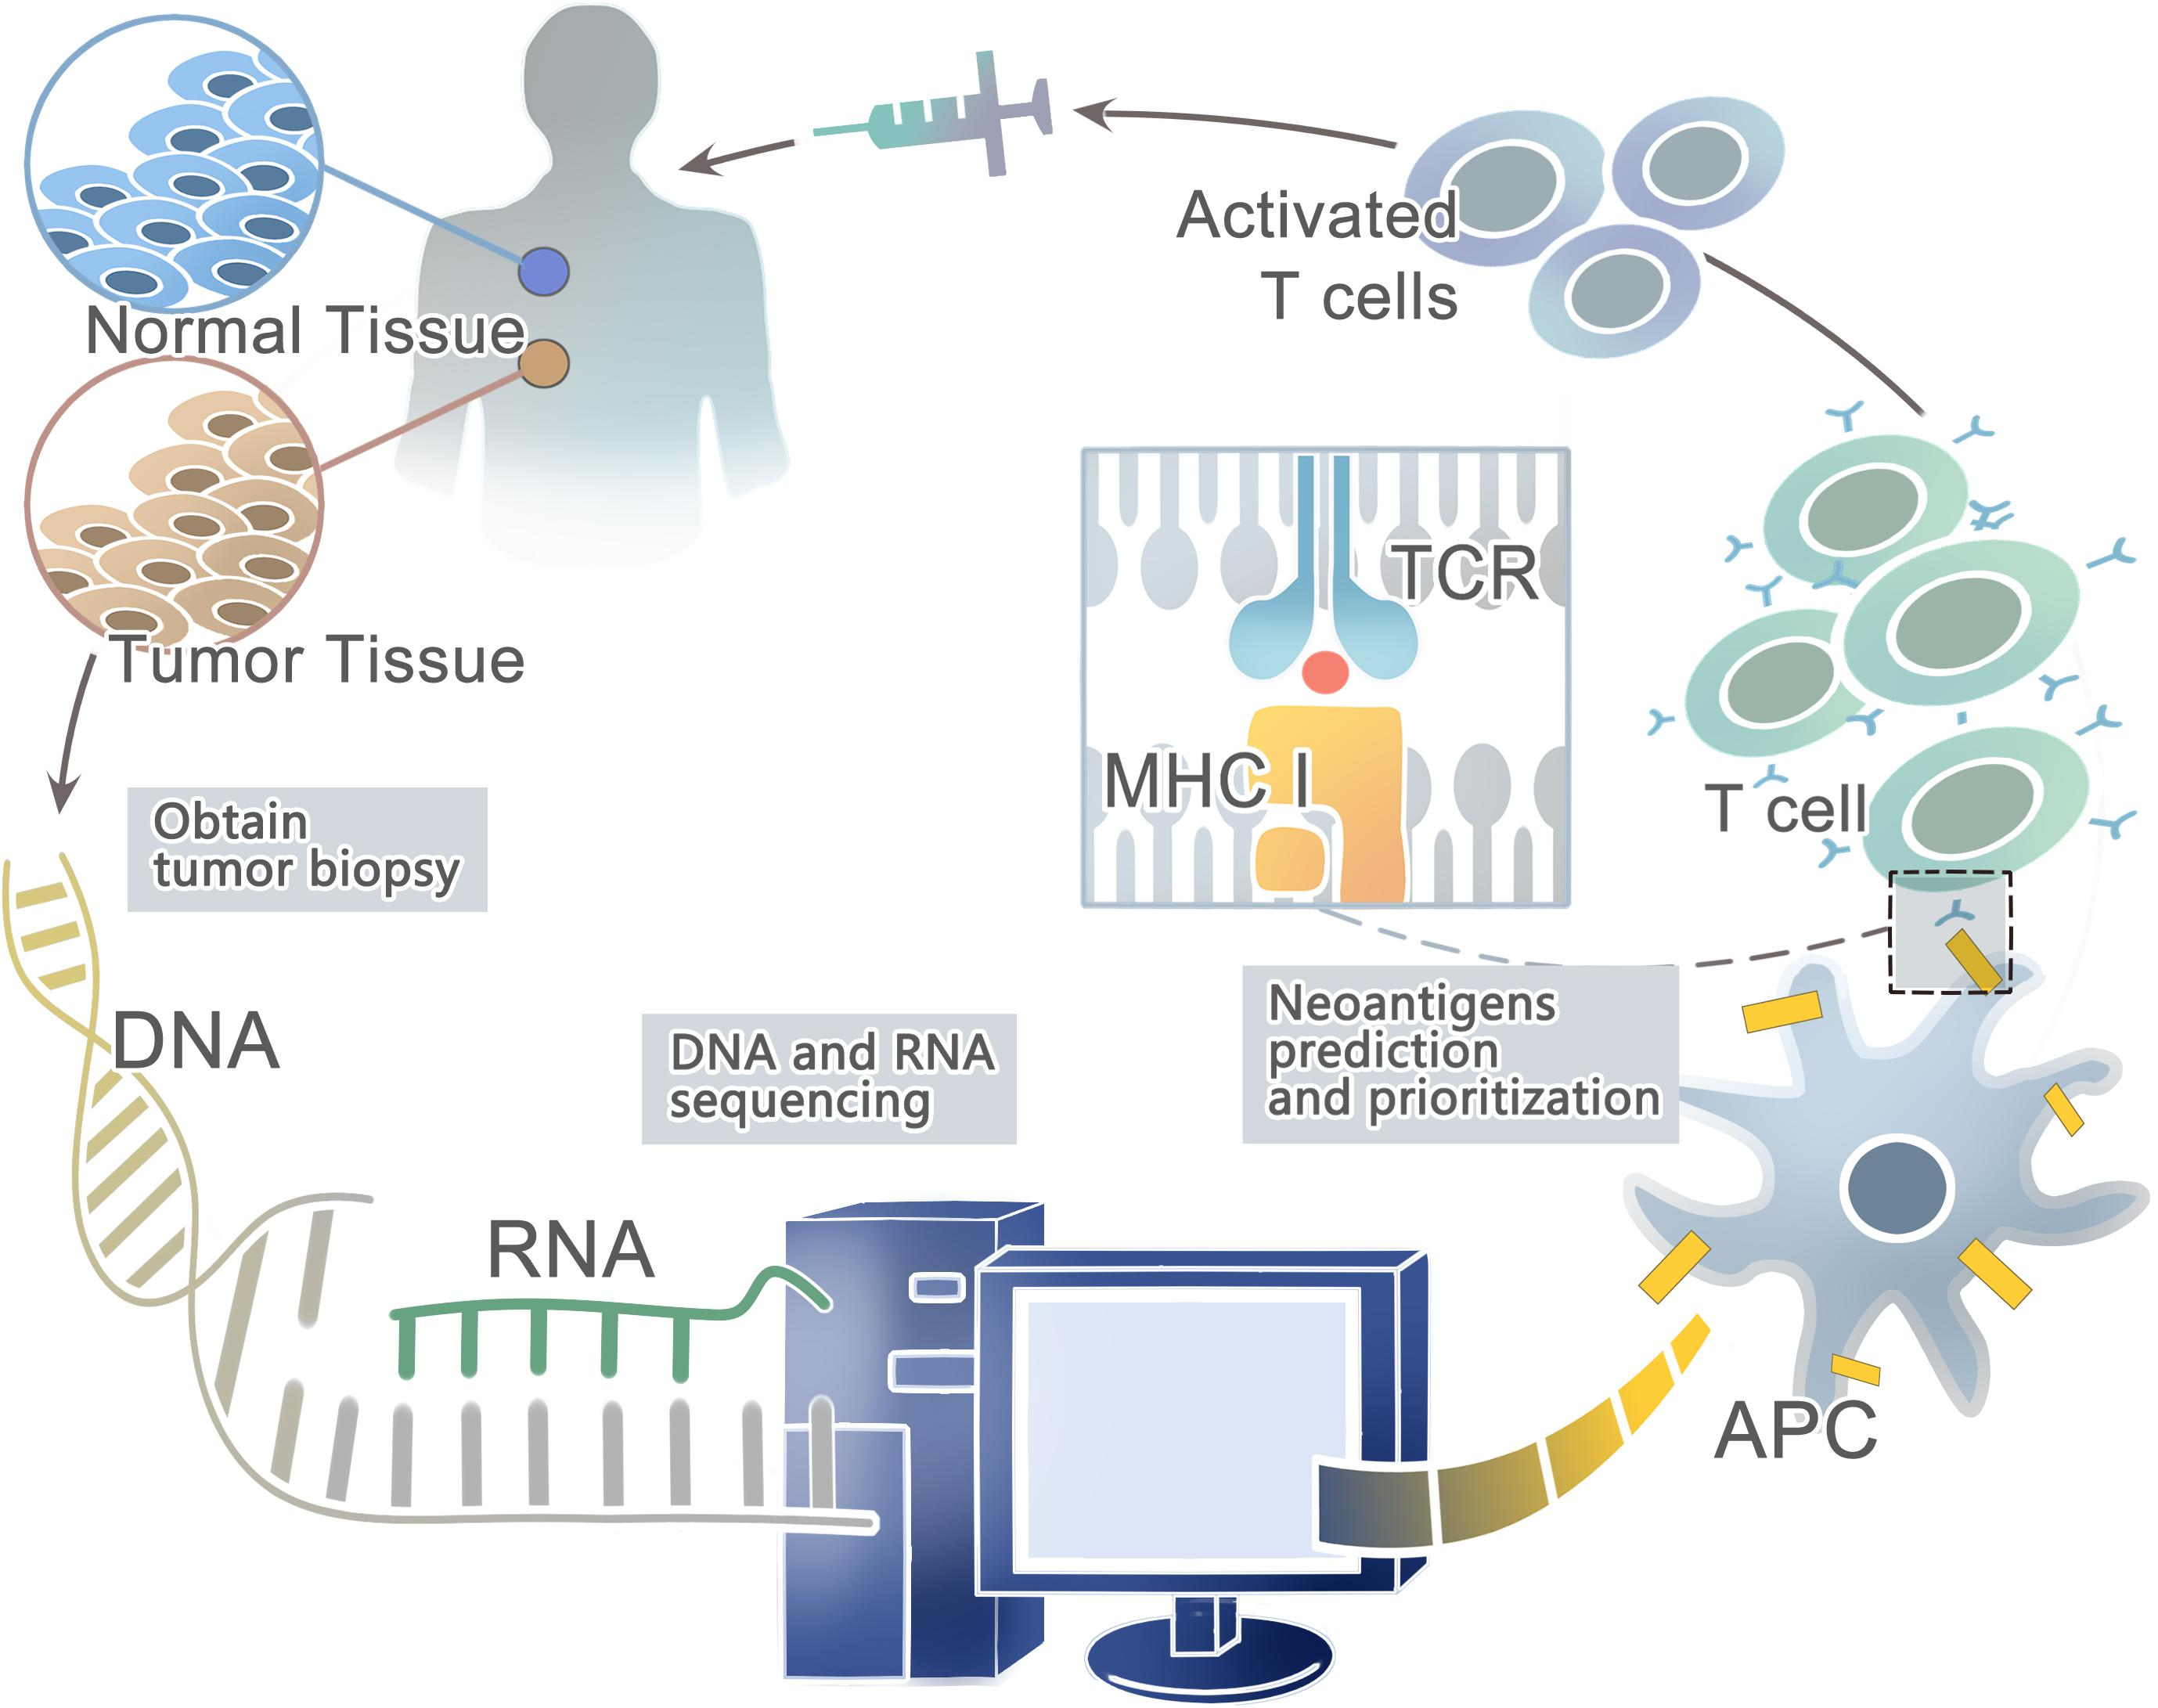
\includegraphics[width=0.8\textwidth]{../img/vaccines/vaccine_pipeline}
		\caption{Proceso de desarrollo de vacunas.}
		\label{fig:vaccines_a}
	\end{subfigure}
	\hfill
	\begin{subfigure}[b]{0.44\textwidth}
		\centering
		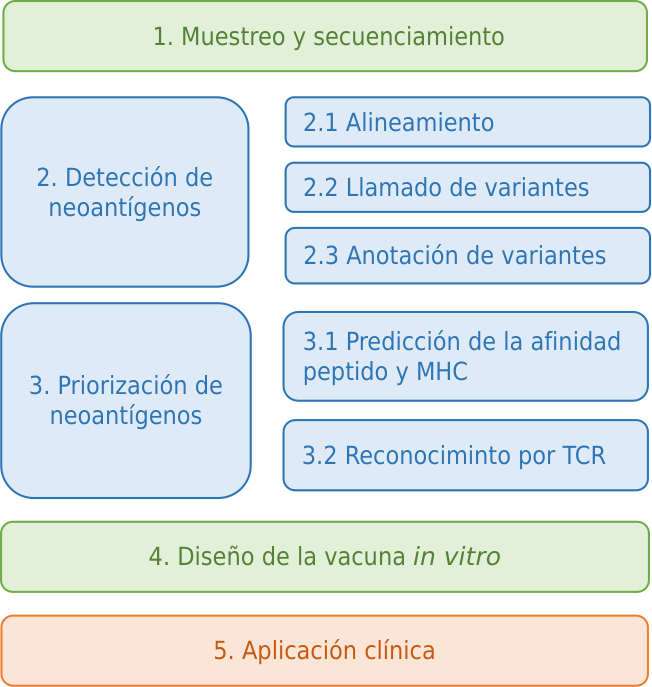
\includegraphics[width=0.8\textwidth]{../img/vaccines/pipeline}
		\caption{\textit{Pipeline} para el desarrollo de vacunas.}
		\label{fig:vaccines_b}
	\end{subfigure}
	
	\caption{Marco de desarrollo para la elaboración de vacunas personalizadas contra el cáncer basadas en neoantígenos. (a) muestra un panorama general de cada etapa. (b) detalla cada fase enfatizando el desarrollo \textit{in-silico}.  Modificado de \cite{han2020progress}.}
	\label{fig:vaccines}
\end{figure}
	
	
La detección \textit{in-silico} de neoantígenos se basa en la segunda y tercera etapa de la Figura \ref{fig:vaccines_b}. En este contexto, debido a la complejidad del proceso y la cantidad de métodos existentes, se han desarrollado software y \textit{pipelines} para facilitar el uso de estas herramientas. En la Tabla \ref{tab:review_pipelines}, presentamos los \textit{pipelines} publicados a partir del 2018. Estos \textit{pipelines} utilizan diferentes tipos de información como entrada, así PGV Pipeline \citep{rubinsteyn2018computational} y PEPPRMINT \citep{zhou2023prioritizing} utilizan DNA-seq; sin embargo, otras herramientas como PGNneo \citep{tan2023pgnneo}, NAP-CNB \citep{wert2021predicting}, NaoANT-HILL \citep{coelho2020neoant}, ProGeo-neo \citep{li2020progeo}, ScanNeo \citep{wang2019scanneo} y Neopepse \citep{kim2018neopepsee} utilizan RNA-seq porque estas secuencias encapsulan mejor la información de mutaciones y \textit{non-coding regions} de ADN \citep{tan2023pgnneo}. 

Con el objetivo de reducir la complejidad de los \textit{pipelines}, otras propuestas han optado por utilizar Variant Calling Format (VCF), como entrada. Estos archivos, contienen información de las mutaciones y son obtenidas a partir de métodos de alineamiento y llamado de mutaciones (etapas 2.1 y 2.2 de la Figura \ref{fig:vaccines_b}). De esta forma, herramientas como Valid-Neo \citep{terai2022valid}, HLA3D \citep{li2022hla3d}, Neoepiscope \citep{wood2020neoepiscope} , pVACtools \citep{hundal2020pvactools} y NeoPredPipe \citep{schenck2019neopredpipe}, reducen la cantidad de herramientas utilizadas en la deteccion de neoantígenos; sin embargo, los resultados obtenidos, pueden ser inferiores comparado con herramientas que usan DNA-seq y RNA-seq.

Adicionalmente, para una correcta detección de neoantígenos, es necesario contar con la secuenciación de proteínas Major Histocompatibility Complex (MHC) o Human Leukocyte Antigens (HLA). Es necesario contar con estas proteínas porque, son utilizadas para predecir la unión entre posibles neoantígenos al MHC (pMHC: etapa 3.1 de la Figura \ref{fig:vaccines_b}). Estas proteínas son codificadas por genes altamente polimórficos, esto proporciona una variación sustancial en la unión de péptidos (neoantígenos), influyendo de esta manera en el conjunto de péptidos presentados a las células T. \citep{abualrous2021major}. En este contexto,  los \textit{pipelines} Valid-NEO \citep{terai2022valid}  y NeoPredPipe \citep{schenck2019neopredpipe} y Neopepsee \citep{kim2018neopepsee} solicitan como entrada estas proteínas (HLA); mientras que las otras predicen esta información a partir de DNA-seq. Desde un punto de vista de usabilidad, obtener los tipos de HLA, implica un esfuerzo inncesario para el usuario.

Es así que se propone el desarrollo de un \textit{pipeline}, que incorpora el uso de MS y fusión de genes. Además, la propuesta incluirá el desarrollo de un modelo \textit{transformers} para la predicción del enlace pMHC y pMHC-TCR. Cabe resaltar, que este proyecto es una continuación del proyecto ``Principales estrategias y métodos basados en deep learning para la detección de neo antígenos en el marco del desarrollo de vacunas personalizadas en la inmunoterapia del cáncer'' financiado por ULaSalle-UCSP, donde se obtuvo dos publicaciones \citep{machaca2023deep,arceda2023neoantigen}. 



%En resumen, el desarrollo de \textit{pipelines} para la detección de neoantígenos es un campo de investigación significativo y de gran envergadura. Además, se está viendo favorecido por el crecimiento exponencial de la información genómica y los avances recientes en inteligencia artificial. 



% falta mencioan porque usan MS


	
\begin{table}[h]
	\caption{Lista de \textit{pipelines} desarrollados desde el 2018 hasta la actualidad para la detección de neoantígenos.GN: Expresión de genes, VA: anotación de variantes.}
	\label{tab:review_pipelines}
 \centering
	\setlength{\tabcolsep}{0.5em} % for the horizontal padding
	{\renewcommand{\arraystretch}{1.5}% for the vertical padding
    {\footnotesize
    \begin{tabular}{lllp{4.5cm}p{2.7cm}}
	\textbf{Nombre} & \textbf{Año}  & \textbf{Ref.}                                 & \textbf{Entrada}                                         & \textbf{Salida}                                     \\ \hline
	
	PEPPRMINT         & 2023 &\cite{zhou2023prioritizing}         & DNA-seq                                                  & Neoantígenos                                        \\

	PGNneo & 2023	& \cite{tan2023pgnneo}	& VCF, RNA-seq y MS data	& Neoantígenos \\
	
	Valid-NEO       & 2022 &\cite{terai2022valid}             & VCF y HLA          & Neoantígenos  \\
	
	HLA3D & 2022	& \cite{li2022hla3d}	& VCF, HLA, SMG y HBV	& Neoantígenos \\
	
	
	
	NAP-CNB         & 2021 &\cite{wert2021predicting}         & RNA-seq                                                  & Neoantígenos                                       \\
	
	NeoANT-HILL     & 2020 &\cite{coelho2020neoant}           & RNA-seq y VCF                        & Neoantígenos,GE  \\
	
	Neoepiscope     & 2020 &\cite{wood2020neoepiscope}        & VCF y BAM                   & Neoantígenos                          \\
	
	ProGeo-neo      & 2020 &\cite{li2020progeo}               & RNA-seq y VCF                        & Neoantígenos                                       \\
	
	pVACtools       & 2020 &\cite{hundal2020pvactools}        & VCF                                         & Neoantígenos                                       \\
	
	NeoPredPipe     & 2019 &\cite{schenck2019neopredpipe}     & VCF y HLA                            & Neoantígenos,VA              \\
	
	ScanNeo         & 2019 &\cite{wang2019scanneo}            & RNA-seq                                                  & Neoantígenos                                       \\
	
		
	Neopepsee       & 2018 &\cite{kim2018neopepsee}           & RNA-seq, VCF, HLA  & Neoantígenos,GE    \\ 
	
	PGV Pipeline    & 2018 &\cite{rubinsteyn2018computational}& DNA-seq                                                  & Neoantígenos                                       \\
	

\end{tabular}
}	
}
\end{table}






%\section{Resultados o avances previos}










\section{Justificación}

El cáncer es el mayor problema de salud mundial; sin embargo, los métodos tradicionales basados en cirugías, radioterapias y quimioterapias tienen baja efectividad \citep{peng2019neoantigen}. En este contexto, los neoantígenos son factores clave en el desarrollo de vacunas contra el Cáncer  \citep{borden2022cancer,chen2021challenges,gopanenko2020main}. Si se logra desarrollar un método con un buen desempeño, la inmunoterapia del cáncer basada en el desarrollo de vacunas personalizadas, podría utilizarse como alternativa a otros métodos como radioterapias y quimioterapias. 

El proyecto tiene dos contribuciones: CONTRIBUCIÓN 01: En el área de ciencia de la computación se va a desarrollar un modelo basado en \textit{transformers} para la predicción del enlace pMHC, actualmente se tienen resultados previos que superan a otros del estado del arte. CONTRIBUCIÓN 02: En el área de la Bioinformática: el desarrollo propio del \textit{pipeline}, representa un reto resolviendo problemas de integración, alto costo computacional, heterogeneidad y modularidad. Además,  el \textit{pipeline} utilizará datos de \textit{Mass Spectrometry} (MS) y fusión de genes para obtener mejores resultados que otros métodos del estado del arte.

Finalmente, el contar con una aplicación de detección de neoantígenos desarrollada por la Universidad La Salle y la Universidad Católica San Pablo, realza el nombre de ambas universidades y demuestra que gracias al trabajo en conjunto se puede desarrollar aplicaciones de gran envergadura aplicadas a campos multidisciplinarios y nos alinea a instituciones como el \textit{European Molecular Biology Laboratory} (EMBL) y el \textit{National Institutes of Health} (NIH).

%\section{Porqué es una investigación básica}
	
%\section{Pregunta de investigación}	
	
\section{Objetivos de la investigación}
	
	\subsection{Objetivo general}
	
	Desarrollar una herramienta  para la detección \textit{in silico} de neoantígenos de cáncer a partir de datos genómicos RNA-seq y DNA-seq.
	
	\subsection{Objetivos específicos}
	\begin{enumerate}
		\item Analizar qué fuentes de información o datos de entrada recibirá la herramienta. Se evaluará DNA-seq, RNA-seq, \textit{Variant Calling File} (VCF) y como integrar esta información con datos de \textit{Mass Spectrometry} (MS).
		
		\item Analizar qué herramientas se utilizarán para la primera etapa de la herramienta, referente al alineamiento de secuencias, llamado de variantes y  anotación de variantes (predicción de posibles neoantígenos). 
		
		\item Analizar el uso de información de variaciones estructurales del ADN y mutaciones de fusión de genes. Se evaluará el desempeño de \textit{Arriba} \citep{uhrig2021accurate} y FusionQ \citep{liu2013fusionq}.

        \item Evaluar métodos de detección de eventos de \textit{alternative splicing} y analizar la aplicación de estos al integrarse a la herramienta para la detección de neoantígenos.
		 
		\item Implementar un modelo basado en \textit{transformers} para la predicción del enlace de los neoantígenos al MHC (pMHC). Ya se cuenta con resultados previos de una propuesta que es superior a otras del estado del arte \citep{arceda2023neoantigen}.

        \item Implementar un modelo basado en \textit{transformers} para la predicción del enlace del enlace pMHC al TCR (pMGC-TCR). 
       
	\item Integrar las herramientas evaluadas en un contenedor Docker.
		
        \item Comparar el desempeño de la herramienta propuesta con otras herramientas del estado del arte.

		
	\end{enumerate}







\section{Metodología} 






Hemos dividido la propuesta en dos módulos: NeoArgosMut y NeoArgosAntigen. NeoArgosMut, se enfoca en el llamado y anotación de variantes, obteniéndose como salida neoantígenos candidatos. Luego, NeoArgosAntigen, prioriza estos antígenos, al predecir su afinidad al MHC (pMHC) y luego la afinidad del pMHC al TCR (pMHC-TCR). En la Figura \ref{fig:pipeline}, mostramos estos módulos. 



\begin{figure}[h]	
		\centering
		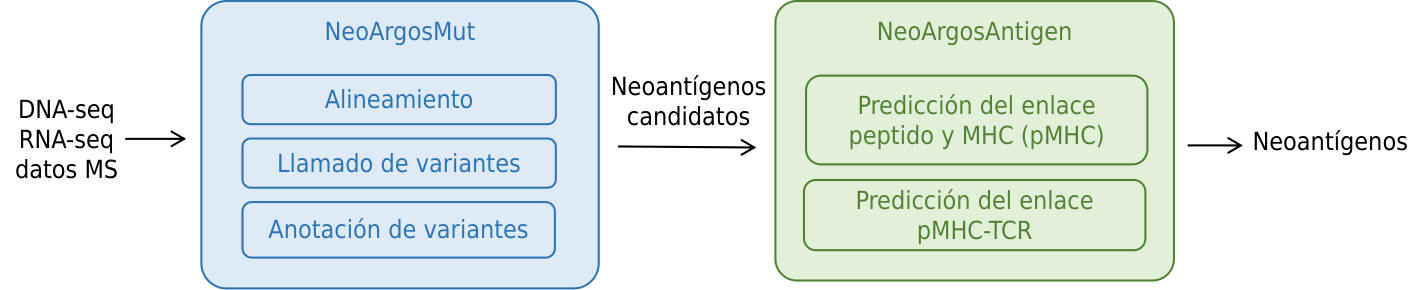
\includegraphics[width=0.8\textwidth]{../img/pipeline/proposal_pipeline}	
	\caption{Representación de NeoArgosMut y NeoArgosAntigen para la detección de neoantígenos}
	\label{fig:pipeline}
\end{figure}


\subsection{NeoArgosMut}

%NeoArgosMut, se encarga de recibir como entrada datos de DNA-seq, RNA-seq y Mass Spectrometry (MS). Luego se plantea alinear dichas secuencias con uso de las herramientas como BWA-MEM \citep{li2013aligning}, Bowtie2 \citep{langmead2012fast}. Adicionalmente, se usará STAR \citep{dobin2013star} porque alinea mejor muestras tumorales \citep{rubinsteyn2018computational}. Como salida a esta etapa, se optiene archivos de alineamiento BAM.

NeoArgosMut, se encarga de recibir como entrada datos de DNA-seq, RNA-seq y Mass Spectrometry (MS). Luego se plantea alinear dichas secuencias con uso de las herramientas como BWA-MEM y Bowtie2. Adicionalmente, se usará STAR, porque alinea mejor muestras tumorales \citep{rubinsteyn2018computational}. Como salida a esta etapa, se optiene archivos de alineamiento BAM.


%Para el llamado de variantes se utilizará MuTect \citep{cibulskis2013sensitive} y Strelka \citep{saunders2012strelka}. Luego, se utilizará la unión de la información de ambos métodos tal como lo hizo \cite{zhou2023prioritizing} y \cite{rubinsteyn2018computational}. Como salida, se obtienen archivos VCF. Adicionalmente a otros \textit{pipelines}, utilizaremos información sobre la fusión de genes que se obtendrán de las herramientas \textit{Arriba} \citep{uhrig2021accurate} y FusionQ \citep{liu2013fusionq}. Esta forma parte de la contribución de este trabajo, porque se sabe que la mayoría de \textit{pipelines} tienen un bajo desempeño debido ausencia de información en su procesos de variantes estructurales y fusión de genes \citep{wood2020neoepiscope}. Finalmente, también se va a utilizar MaxQuant \citep{cox2008maxquant} para identificar las mutaciones a nivel de péptidos con ayuda de información de Mass Spectrometry (MS), esto también forma parte de la contribución del trabajo al incluir fuentes adicionales de información como MS.

Para el llamado de variantes se utilizará MuTect y Strelka. Luego, se utilizará la unión de la información de ambos métodos tal como lo hizo \cite{zhou2023prioritizing} y \cite{rubinsteyn2018computational}. Como salida, se obtienen archivos VCF. Adicionalmente a otros \textit{pipelines}, utilizaremos información sobre la fusión de genes que se obtendrán de las herramientas \textit{Arriba} \citep{uhrig2021accurate} y FusionQ \citep{liu2013fusionq}. Esta forma parte de la contribución de este trabajo, porque se sabe que la mayoría de \textit{pipelines} tienen un bajo desempeño debido ausencia de información en su procesos de variantes estructurales y fusión de genes \citep{wood2020neoepiscope}. Finalmente, también se va a utilizar MaxQuant para identificar las mutaciones a nivel de péptidos con ayuda de información de Mass Spectrometry (MS), esto también forma parte de la contribución del trabajo al incluir fuentes adicionales de información como MS.


%Luego corresponde a la anotación de variantes, en esta etapa se toman los archivos en formato VCF y se obtienen los péptidos generados a partir de estas variaciones o mutaciones. Estos péptidos representan los posibles neoantígenos. Para está tarea se va a utilizar Isovar y ANNOVAR \citep{wang2010annovar}. 
Luego corresponde a la anotación de variantes, en esta etapa se toman los archivos en formato VCF y se obtienen los péptidos generados a partir de estas variaciones o mutaciones. Estos péptidos representan los posibles neoantígenos. Para está tarea se va a utilizar Isovar y ANNOVAR. 

%Finalmente, para obtener el tipo de HLA del paciente se va a utilizar la herramienta OptiType \citep{szolek2014optitype}. Otros \textit{pipelines} optan por solicitar al usuario la información del tipo de HLA; sin embargo, obtener el HLA a partir de las mismas secuencias de ADN, mejora considerablemente el desempeño general del pipeline y la accesibilidad del usuario. 
Finalmente, para obtener el tipo de HLA del paciente se va a utilizar la herramienta OptiType. Otros \textit{pipelines} optan por solicitar al usuario la información del tipo de HLA; sin embargo, obtener el HLA a partir de las mismas secuencias de ADN, mejora considerablemente el desempeño general del pipeline y la accesibilidad del usuario. Al  finalizar esta etapa, se va a obtener los neoantígenos candidatos.


\subsection{NeoArgosAntigen}

NeoArgosAntigen, prioriza los neoantígenos detectados previamente por NeoArgosMut. Esta priroización la realiza en base a la predicción del enlace de los neoantígenos al MHC y posteriormete al TCR. El módulo se divide en dos partes: la predicción del enlace pMHC y la afinidad del pMHC al TCR. Ambas toman como entrada dos secuencias de proteínas, luego se necesita predecir su afinidad (regresión) o el enlace (clasificación). En resumen, las proteínas se pueden representar como $p = \{ A, ... , Q \}$ y $q = \{ A, N, ... ,Q, E, G \}$. Luego, tenemos que  predecir la probabilidad del enlace o afinidad entre $p$ y $q$. 

\begin{wrapfigure}{r}{0.48\textwidth} %this figure will be at the right
    \centering
    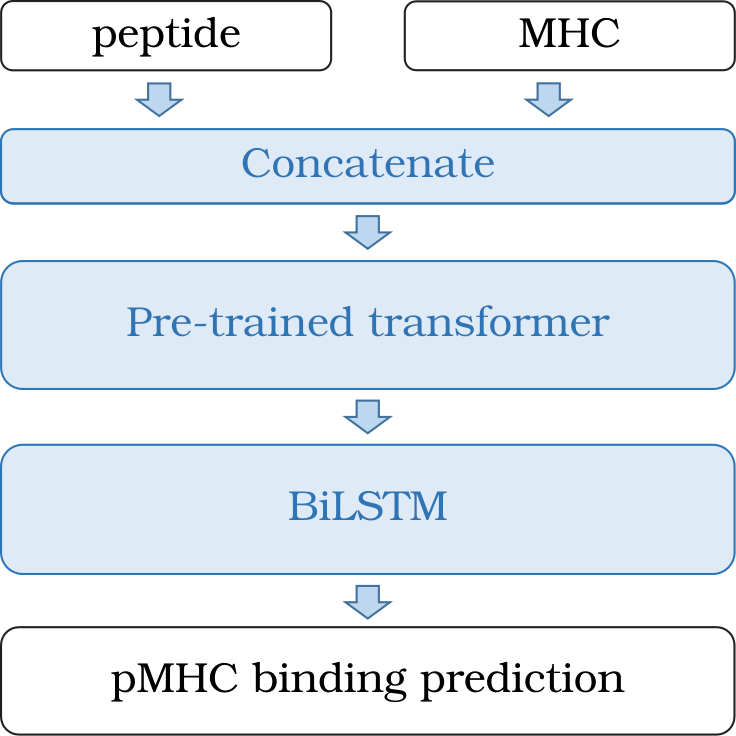
\includegraphics[width=0.30\textwidth]{../img/pipeline/proposal_pmhc}
    \caption{Modelo  \textit{transformer} seguido de BiLSTM para predecir el enlace pMHC.}
	\label{fig:proposal}
\end{wrapfigure}

Para el problema de predicción del enlace pMHC se va a utilizar modelos BERT pre-entrenados y se realizará \textit{fine-tuning} agregando un bloque de capas BiLSTM. Luego se volverá a entrenar estos modelos con una base de datos compuesta por muestras de \cite{zhang2022hlab} y \cite{gfeller2023improved}. Se propone la arquitectura de la Figura \ref{fig:proposal}. Como se puede ver, la entrada son dos secuencias de proteínas: el péptido y el MHC. Luego, el modelo basado en transformers está compuesto por un modelo pre-entrenado y un bloque de capas BiLSTM, esta propuesta se basó en el trabajo de \cite{zhang2022hlab}. En esta etapa también. se va a evaluar el desempeño de varios modelos BERT pre-entrenados como: TAPE \citep{rao2019evaluating}, ProtBERT-BFD \citep{elnaggar2021prottrans} y ESM2 \citep{lin2023evolutionary} cada una con 92 millones, 420 millones, 650 millones parámetros respectivamente. Adicionalmente, TAPE fue entrenado con 30 millones de proteínas, ProtBERT-BFD con 2122 millones de proteínas y 60 millones de proteínas para ESM-2. En base a trabajos anteriores propios, sabemos que el uso de TAPE y el modelo más pequeño de ESM2 tienen buenos resultados \citep{arceda2023neoantigen}.




%  \begin{figure}[H]
%	\centering
%	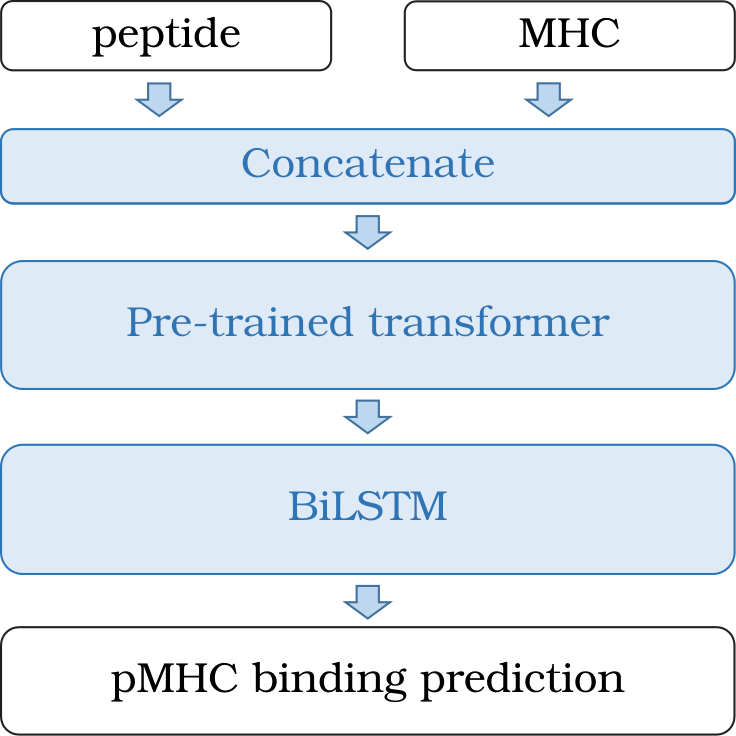
\includegraphics[width=0.30\textwidth]{../img/pipeline/proposal_pmhc}
%	\caption{Propuesta: Utilizamos el modelo de transformer ESM2 seguido de BiLSTM para predecir el enlace pMHC.}
%	\label{fig:proposal}
%\end{figure}





La misma arquitectura de la Figura \ref{fig:proposal}, se utilizará para la predicción del enlace pMHC y TCR (pMHC-TCR) según recomendaciones de \cite{li2020progeo}  y \cite{myronov2023bertrand}. Sin embargo, se va reentrenar el modelo para adaptarse a este nuevo problema, se utilizarán muestras de \cite{li2020progeo} y la base de datos de VDJdb \citep{shugay2018vdjdb}. Al finalizar esta etapa, se obtendrán los neonatígenos.





%\section{Limitaciones}

%\section{Describa el equipamiento e infraestructura disponible}

%\section{Resultados esperados}

%\section{Cronograma de Actividades}

%\section{Sostenibilidad de la propuesta}

%\section{Impacto Científico de la propuesta}






\bibliographystyle{apalike}
\bibliography{bibliography}

	
\end{document}